% Raoul Rubien 2016
% template based on 
% Time-stamp: <2004-06-26 17:18:02 mp>
% Authors: The LaTeX@TUG-Team [http://latex.tugraz.at/]:

\documentclass[
a4paper,
parskip, % empty line between two paragraphs
%draft, % en-/disable draft
DIV14, % enlarges the pages
11pt,
]{scrartcl}

\usepackage[
colorinlistoftodos,
prependcaption,
textsize=tiny,
% disable % en-/disable todos globally
]{todonotes}

% by modifying the page margins the total page number can be minimally adjusted
\usepackage[scale=0.8]{geometry} % adjust page margins

\usepackage{tikz}
\usetikzlibrary{calc}

\usepackage{ifdraft} % http://mirror.easyname.at/ctan/macros/latex/contrib/oberdiek/ifdraft.pdf
\ifdraft{\usepackage{showframe}}{} % on draft option enabled show frames

% compilation output language setup: enable the respecive optional package
\usepackage[
%de, % compile to german output
 en, % compile to english output
]{optional} 

\opt{de}{
  \usepackage[latin1]{inputenc}
  \usepackage[T1]{fontenc}
  \usepackage[ngerman]{babel}
  % additional language specific hyphenation can be added here
  \hyphenation{Pro-gram-mier-me-tho-den}
}
\newcommand{\de}[1]{\opt{de}{#1}} % convenience macro
\opt{en}{
	\usepackage[latin1]{inputenc}
    \usepackage[T1]{fontenc}
	\usepackage[american]{babel}
    % additional language specific hyphenation can be added here
}
\newcommand{\en}[1]{\opt{en}{#1}} % convenience macro

\newcommand{\myDocumentTitle}{curriculum vit{\ae}}
\newcommand{\myDocumentAuthor}{Noodly~Monster, \de{MSc}\en{Dipl.-Ing.}}

\usepackage{ae,aecompl}

\usepackage{currvita} % http://mirror.easyname.at/ctan/macros/latex/contrib/currvita/currvita.pdf
\renewcommand*{\cvheadingfont}{\raggedleft\Huge\bfseries} % currvita settings for headings

\usepackage[
% pdftex=true,
colorlinks=true,
%pdfstartpage={1}, % on which page the PDF is opened
]{hyperref} % http://mirror.easyname.at/ctan/macros/latex/contrib/hyperref/doc/manual.pdf

% setting pdf meta data
\hypersetup{
  pdftitle={\myDocumentTitle},
  pdfauthor={\myDocumentAuthor},
  pdfsubject={\myDocumentTitle},
  pdfcreator={}
  pdfproducer={\myDocumentAuthor},
  pdfkeywords={\myDocumentTitle, \myDocumentAuthor}
}

\emergencystretch 1.5em % no words should exceed the line:

\renewcommand{\familydefault}{\sfdefault} % set sans serif font for whole document

% frequently used terms in both langages
\newcommand{\myEducationalInstitution}{\de{Bildungseinrichtung}\en{Educational Institution}}
\newcommand{\myInstitution}{\de{Einrichtung}\en{Institution}}
\newcommand{\myTopic}{\de{Thema}\en{Topic}}
\newcommand{\myFocus}{\de{Fokus}\en{Focus}}
\newcommand{\mySelfEmployed}{\de{Selbstst�ndig}\en{Self-employed}} 
\newcommand{\myUniversity}{\de{Pastafari Universit�t Oregano}\en{Pastafarian University of Oregano}}
\newcommand{\myOtherUniversity}{\de{Universit�t Oregano}\en{Oregano State University}}
   
% convenience macros
\newcommand{\myItem}{\item}
\newcommand{\mySubitem}{\subitem $\circ$\ }

\begin{document}
\normalsize
%\thispagestyle{empty} % en-/disable page numbering on this page


\begin{cv}{\myDocumentTitle}
    \begin{tikzpicture}[remember picture,overlay]
       % modify the "-(Xem,Yem)" parameter to adjust the position of your photo 
        \node[anchor=north east,inner sep=0pt] at ($(current page.north east)-(5em,8.75em)$) {
            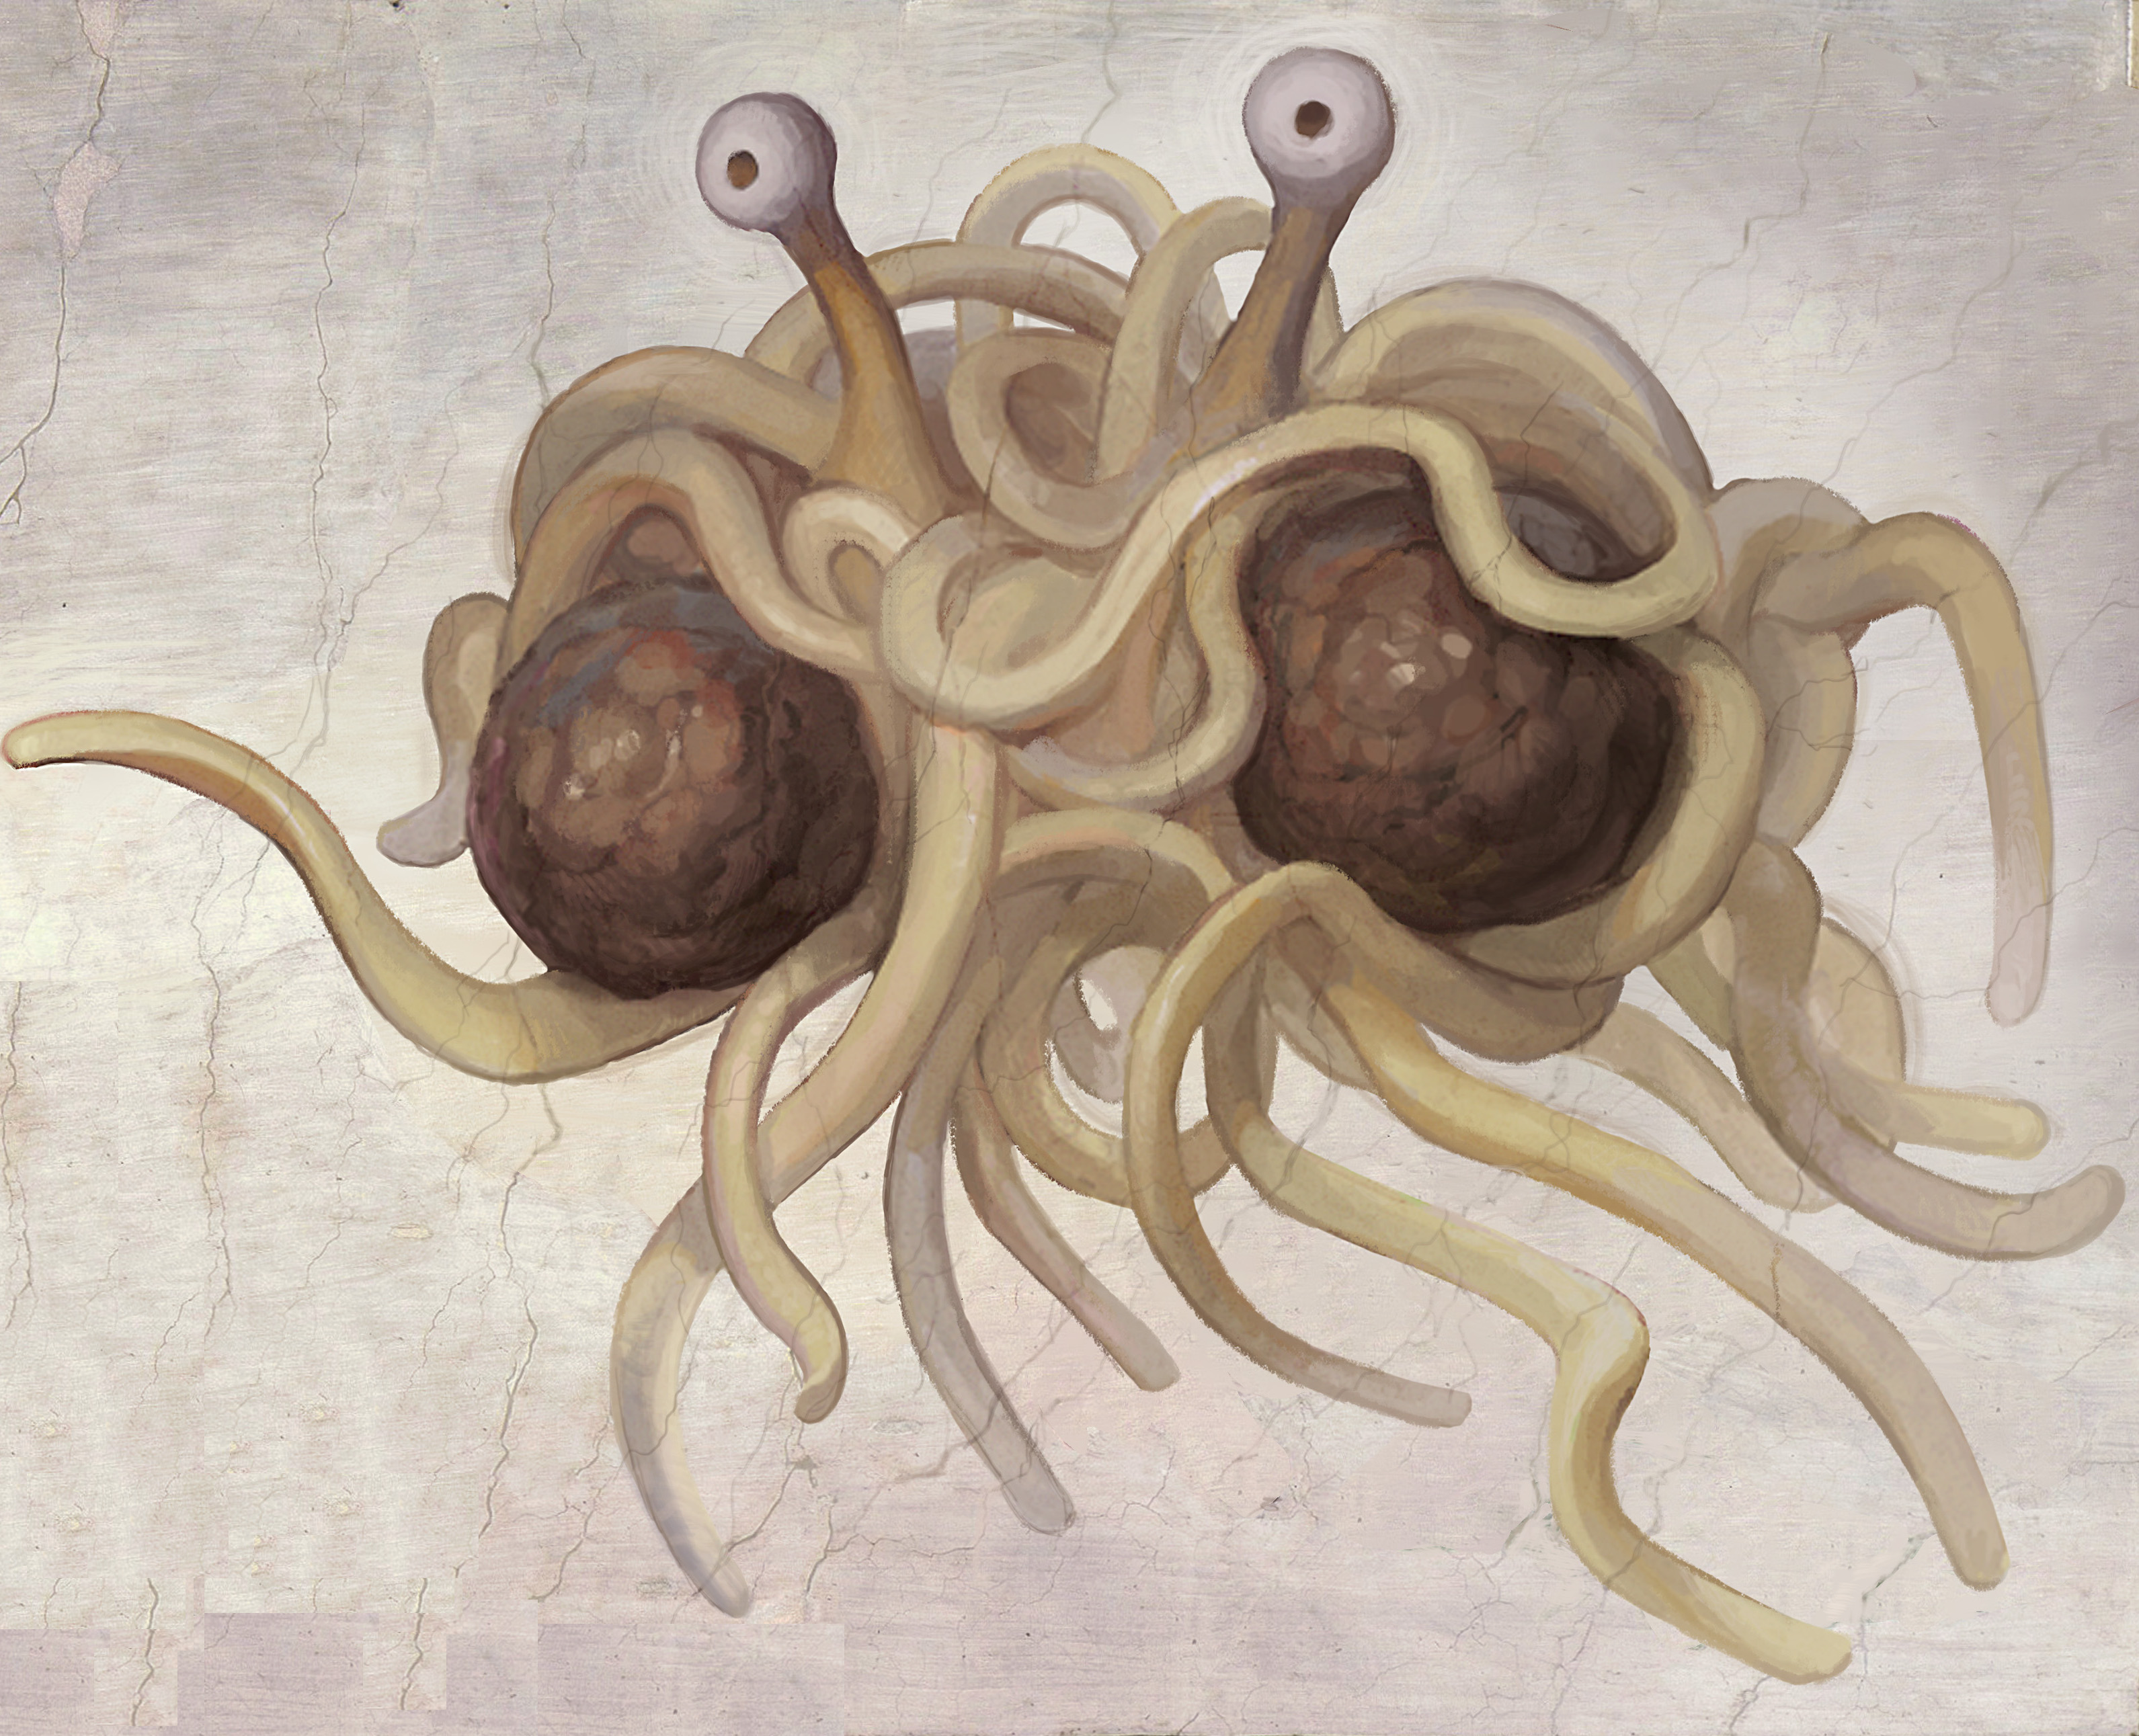
\includegraphics[width=0.3\textwidth,]{./touched_by_his_noodly_appendage}
    	};
    \end{tikzpicture}
	% set the width of the first column to the widest entry
	\settowidth{\cvlabelwidth}{\cvlabelfont Spezielle Kenntnisse}

    \begin{cvlist}{\myDocumentAuthor}
        \item[\de{Geboren~am}\en{Date of Birth}]
            \de{1. Januar 2005}
            \en{January 1\textsuperscript{st} 2005}
    
        \item[\de{Familienstand}\en{Marriage Status}]
            \de{Ledig}
            \en{Single}
        
        \item[\de{Staatsb�rgerschaft}\en{Nationality}]
            \de{�sterreich}
            \en{Austria}
        
        \item[\de{Adresse}\en{Address}]
            \de{Hintertupfing 13/2\\A-1920 Salzhausen}
            \en{Behinddapple 13/2\\1920 Salthausen, Austria}
        
        \item[\de{E-Mail Adresse}\en{E-Mail}]
            noodly.monster@student.pastauniversity.at
        
        \item [\de{Telefonnummer}\en{Phone}]
            +43 (0)190 888 6969
            
        \item[\de{F�hrerschein}\en{Driving License}]
            \de{A, B}
            \en{A (motorcycle), B (car)}
        
        \item[\de{Sprachen (GERS)}\en{Languages (CEFR)}]
            \de{Deutsch (Muttersprache, C2), Sarkasmus (in Wort und Schrift, C1)}
            \en{English (mother tongue, C2), Sarcasm (in speech and writing, C1)}
    \end{cvlist}

   \todo{Mention your hightest degree here instead of the (normal) education listing.
    Explicitely mention the institution. in austria this means University, Fast\-hoch\-schule, Html or Matura.
     Also mention the title and extent of your work}
    \begin{cvlist}{\de{Ausbildung}\en{Education}}
        \item[2015-2016]
            \de{Pastafarismus-Wirtschaft, Dipl.-Ing.\\
                \textbf{\myEducationalInstitution:} \myUniversity, Oregon\\
                \textbf{\myTopic:} Piraten und die Globale Erw�rmung\\
                \textbf{\myFocus:} Eine detailierte Undtersuchung der Korrelation zwischen Anzahl lebender Piraten und der Erdew�rmung.}
            \en{Pastafarism and Management, MSc (Dipl.-Ing.)\\
                \textbf{\myEducationalInstitution:} \myUniversity, Oregon\\
                \textbf{\myTopic:} Pirates and the Global Warming\\
                \textbf{\myFocus:} A deep survey on the correlation between the number of pirates with global temperature.}
            
        \item[2014-2015] 
            \de{Pastafarismus-Wirtschaft, BSc\\
                \textbf{\myEducationalInstitution} \myUniversity, Oregon\\
                \textbf{\myTopic:} Studie �ber das Kochen von Fliegenden Nudeln\\
                \textbf{\myFocus:} Eine Evaluierung g�nstiger Nudelsiebe.}
            \en{Pastafarism and Management, BSc\\
                \textbf{\myEducationalInstitution}: \myUniversity, Oregon\\
                \textbf{\myTopic:} Study on how to Cook Flying Noodles\\
                \textbf{\myFocus:} An evaluation of low cost noodle colander}
    \end{cvlist}
    \todo{Your job history.}
    \begin{cvlist}{\de{Berufserfahrung}\en{Career}}%Employment}}
        \item[2013-2014] 
            \de{Gottheit}
            \en{Deity}\\
            \myInstitution: \mySelfEmployed, Milky Way
        
        \item[2012-2013] 
            \de{Priester}
            \en{Priest}\\
            \myInstitution: Church of the Flying Spaghetti Monster, Oregon
            
        \item[2011-2012] 
            \de{Flugschein}
            \en{Pilot's license}\\
            \myInstitution: Acme GmbH (Noodly Center for Flying Monsters \& Meatballs), Oregon
            
        \item[2010-2011]
            \de{Bildungskarenz}
            \en{Paid leave for further training or education}
             
        \item[2008-2009]
            \de{EDV-Leistungen: Installation, Datenrettung, Instandhaltung, Organisation etc. f�r Privatpersonen und Firmen}
            \en{EDP-Services: Installation, data recovery, maintenance, organization etc. for private persons and companies}\\
            \myInstitution: \mySelfEmployed
            
        \item[2007] 
            \de{M�llmann (Ferialpraktikum)}
            \en{Garbage collector (holiday internship)}\\
            \myInstitution: Oregon City Garbage Co., Oregon
    \end{cvlist}
    \todo{Mention your special interest i.e.: programming languages, hobbies, sports, et cetera.}
    \begin{cvlist}{\de{Spezielle Kenntnisse}\en{Special Interests}}
        \myItem[Cooking] ~
            \mySubitem \de{Nudeln}\en{Noodles}
            \mySubitem \de{Fleschkl��chen}\en{Meat balls}

        \item[\en{Professional pastafarian protester}\de{Professioneller Pastafari Protestant}] ~
        
        \myItem[Programming] ~
            \mySubitem PHP, JavaScript, XML, HTML 1.0
        
        \item[\de{Hobbys}\en{Hobbies}] ~
            \mySubitem 
                \de{Leute mit meinem nudeligen K�rperteil ber�hren}
                \en{Touching people with my noodly appendage}
            \mySubitem
                \de{Nudelsieb als Kopfschmuck tragen}
                \en{Wearing colander headdress}
            \mySubitem
                \de{Pastafarismus}
                \en{Pastafarism}
    \end{cvlist}
    
    \todo{Explicitly mention your off-topic skills. I.e. for a software engineer it's the soft skills}
    \begin{cvlist}{\de{Sozialkompetenz}\en{Soft Skills}}
        \item[2014]
            \de{Projektcontrolling}
            \en{\en{Project Controlling}}\\
            \myEducationalInstitution: \myUniversity, Oregon
        
        \item[2014]
            \de{Mitarbeiterf�hrung von Piraten}
            \en{Leadership of Pirates}\\
            \myEducationalInstitution: \myOtherUniversity, Oregon
        
        \item[2013]
            \de{Konfliktmanagement (Piratengrundkurs)}
            \en{Conflict Management (elementary pirate level)}\\
            \myEducationalInstitution: \myOtherUniversity, Oregon
    \end{cvlist}
    
    \todo{Exclusive or voluntary education that does not belong to your study.}
    \begin{cvlist}{\de{Studium und Weiterbildung}\en{Studies and Trainings}}
        \item[2012] 
            \de{Marketing \& Propaganda}
            \en{Marketing \& Propaganda}\\
            \myEducationalInstitution: \myUniversity, Oregon
            
        \item[2011]
            \de{Lehrwerkst�tte - Nudeln, Fleischkl��chen, Saucen}
            \en{Training Workshop - Noodles, Meatballs, Sauces}\\
            \myEducationalInstitution: \myUniversity, Oregon
            
        \item[2010]
            \de{Grundkurs zum Piratenbraumeister}
            \en{Pirate Master Brewer (elementary level)}\\
            \myEducationalInstitution: \myUniversity, Oregon     
    \end{cvlist}
    
    \todo{You normal education.}
    \begin{cvlist}{\de{Schulische Ausbuilding}\en{Educational Training}}
        \item[2008-2009] 
            \de{Pastafari Realgymnasium (Oberstufe), Hintertupfing}
            \en{Pastafarian High school, Behinddapple}
            
        \item[2007-2008]
            \de{Pastafari Mittelschule, Behinddapple}
            \en{Pastafarian Middle school, Hintertupfing}
        
         \item[2006-2007] 
             \de{Volksschule, Behinddapple}
             \en{Elementary school, Hintertupfing}
         
         \item[2005-2006] 
             \de{Vorschule, Behinddapple}
             \en{Preschool, Hintertupfing}
    \end{cvlist}
  
     \todo{Declare your publications if you have any.}
    \begin{cvlist}{\de{Publikationen}\en{Publications}}
        \item[2006]
            \textbf{Noodly Monster}, Henderson, Bobby. The gospel of the flying spaghetti monster. New York: Villard Books, 2006. Print.
    \end{cvlist}

    \de{\cvplace{Oregon} \date{18. Dezember 2016}}
    \en{\cvplace{Oregon} \date{December 18\textsuperscript{th} 2016}}
\end{cv}
\end{document}